
\documentclass[a4paper,oneside,12pt]{article}

\usepackage[utf8]{inputenc}    % make čšž work on input
\usepackage[T1]{fontenc}       % make čšž work on output
\usepackage[slovene]{babel}    % slovenian language and hyphenation
\usepackage[reqno]{amsmath}    % basic math
\usepackage{amssymb,amsthm}    % math symbols and theorem environments
\usepackage{graphicx}          % images
\usepackage{enumerate}
\usepackage{physics}
\usepackage[
  paper=a4paper,
  top=2.5cm,
  bottom=2.5cm,
  left=2.5cm,
  right=2.5cm
% textheight=24cm,
]{geometry}  % page geomerty

% vstavi svoje pakete tukaj
\usepackage{fancyhdr}
\usepackage{tikz}
\usepackage{makeidx}
\makeindex
\usepackage[all]{xy}
% \usepackage{minted}
\usepackage{pythonhighlight}
  % algorithms
  \RequirePackage{algpseudocode}  % za psevdokodo
  \RequirePackage{algorithm}      % za plovke
  \floatname{algorithm}{Algoritem}
  \renewcommand{\listalgorithmname}{Kazalo algoritmov}
%  \algnewcommand\algorithmicto{\textbf{to}}
%  \algnewcommand\algorithmicin{\textbf{in}}
%  \algnewcommand\algorithmicforeach{\textbf{for each}}
%  \algrenewtext{For}[3]{\algorithmicfor\ #1 $\gets$ #2\ \algorithmicto\ #3\ \algorithmicdo}
%\algdef{S}[FOR]{ForEach}[2]{\algorithmicforeach\ #1\ \algorithmicin\ #2\ \algorithmicdo}


% clickable references, pdf toc
\usepackage[bookmarks, colorlinks=true, linkcolor=black, anchorcolor=black,
  citecolor=black, filecolor=black, menucolor=black, runcolor=black,
  urlcolor=black, pdfencoding=unicode]{hyperref}

\setlength{\parindent}{0pt}    % zamik vsakega odstavka
\setlength{\parskip}{10pt}     % prazen prostor pod odstavkom
% lastne definicije
\newcommand{\N}{\ensuremath{\mathbb{N}}}
\newcommand{\Z}{\ensuremath{\mathbb{Z}}}
\newcommand{\Q}{\ensuremath{\mathbb{Q}}}
\newcommand{\R}{\ensuremath{\mathbb{R}}}
\renewcommand{\C}{\ensuremath{\mathbb{C}}}
% stavi lastne definicije tukaj
\newcommand{\dpar}[2]{\frac{\partial #1}{\partial #2}}
  \floatname{listing}{Koda}
  \renewcommand{\listalgorithmname}{Kazalo programske kode}
% \pagestyle{empty}              % vse strani prazne (ni okraskov, številčenja....)
% \setlength{\parindent}{0pt}    % zamik vsakega odstavka
% \setlength{\parskip}{10pt}     % prazen prostor pod odstavkom
%\setlength{\overfullrule}{30pt}  % oznaci predlogo vrstico z veliko črnine
\frenchspacing % to se priporoča, da bo presledek za piko na koncu stavka enako dolg kot obični.
%Alternativa je ročno metanje \ za vsako okrajšavo.
\newcommand{\td}[2]{\frac{\mathrm{d}{ #1}}{\mathrm{d}{ #2}}}
\hypersetup{pdftitle={Modelska 206}, pdfauthor={Peter Rupnik}} %To piše v pdf viewerju na vrhu! veri neat
\title{206: Parcialne diferencialne enačbe: lastne rešitve}
\author{Peter Rupnik}
\def\thesection{\arabic{section}. naloga}
\def\thesubsection{\arabic{section}.\arabic{subsection}}
\begin{document}
\maketitle
\section{}

Določi nekaj najnižjih lastnih frekvenc in lastnih nihanj kvadratne opne, ki je odebeljena na večjo ploskovno gostoto povsod, kjer je slika spodaj senčena sivo. Prevedi problem na sistem diferenčnih enačb. Kaj pa, če je senčeno območje lažje? Oglej si odvisnost spektra od gostote sivega polja.
\begin{center}
    
\includegraphics[width=0.5\textwidth]{1-figura.pdf}
\end{center}
Poleg direktne diagonalizacije preskusi še metodo z inverzno iteracijo. Ker je matrika redka in nas zanima le prvih nekaj lastnih vrednosti in vektorjev, lahko uporabiš tudi knjižnice za delo z redkimi matrikami.
Konvergenco, hitrost in natančnost metod preskusi na neobteženi opni.


\subsection{Tipanje problema}
Pričel sem z neokrnjeno, kvadratno \emph{tabulo raso}. Uveril sem se, da znam poiskati lastne nihajne načine in pripadajoče lastne vrednosti. Po pripravi matrike $A$ sem ugotovil, da metoda \texttt{scipy.linalg.eigh} deluje odlično, metode iz naprednejšega modula \texttt{scipy.sparse.linalg} pa so malenkost zahtevnejše, vendar s pravo optimizacijo parametrov povrnejo ekvivalentne rezultate.

Prvih nekaj lastnih vrednosti prikazujem spodaj. Opazimo, da lastne vrednosti ležijo druga na drugi, ker pa imajo vsake oči svojega malarja, sem preveril še numerično ekvivalenco obeh vektorjev lastnih vrednosti:
\begin{python}
np.allclose(eigenvalues_sparse[:16], eigenvalues[:16])
True
\end{python}
\begin{center}
    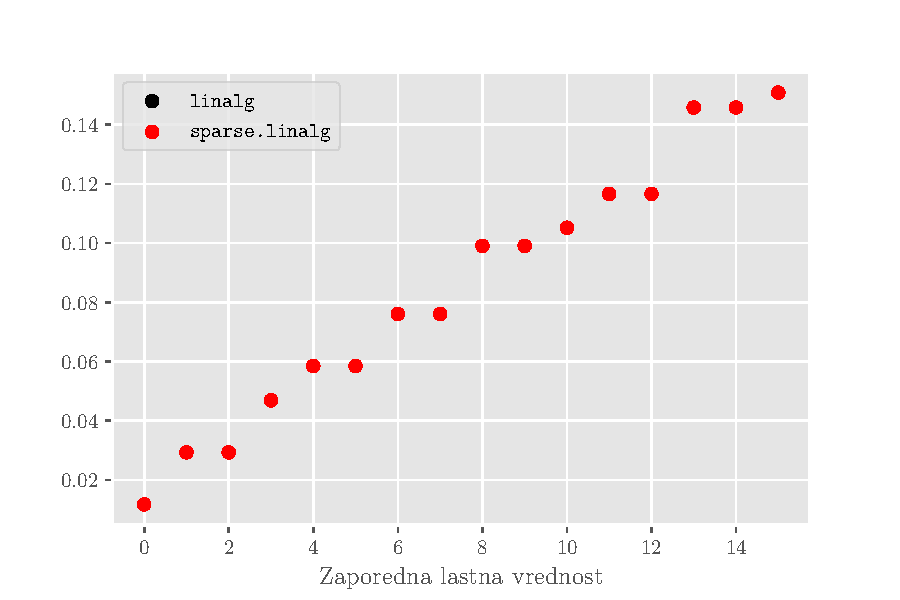
\includegraphics[width=0.7\textwidth]{1-0-spekter-zoom.pdf}
\end{center}
Če nadaljujemo raziskovanje lastnih vrednosti vse do višjih, dobim ponovno ekvivalenco naračunanih lastnih vrednosti. Izgled polnega spektra prikazujem spodaj:
\begin{center}
    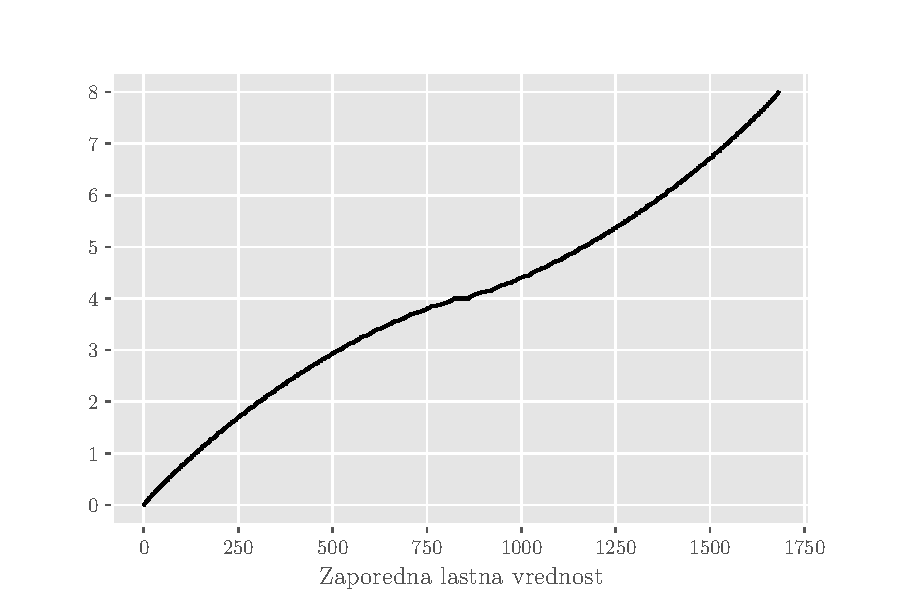
\includegraphics[width=0.7\textwidth]{1-0-spekter.pdf}
\end{center}
Akademska radovednost veli, da izrišemo vsaj nekaj osnovnih nihajnih načinov,  ki jih porodita obe metodi. Za 'klasično' metodo, ki ne upošteva posebnih odlik vhodne matrike, dobim sledečo sliko.
\begin{center}
    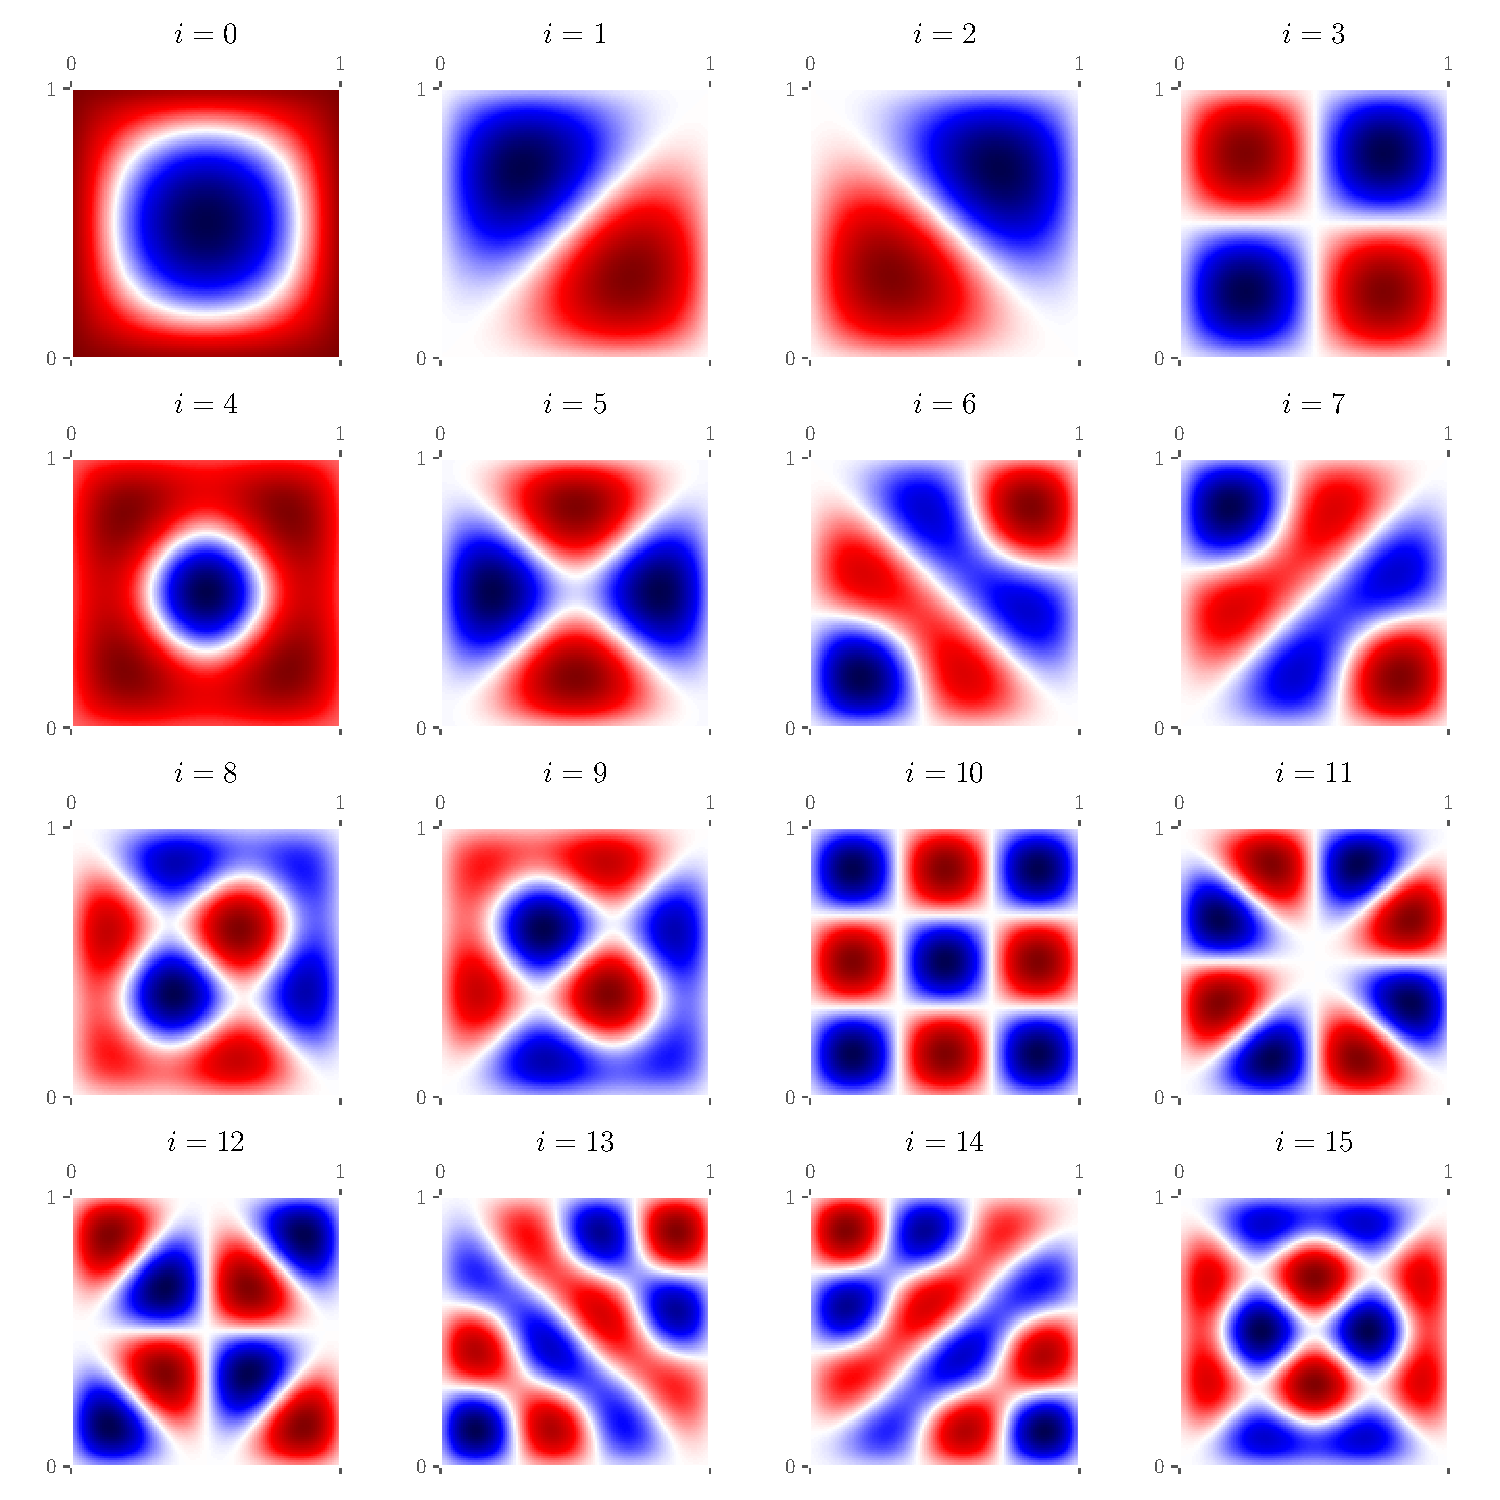
\includegraphics[width=0.7\textwidth]{1-0-nihajni_nacini.pdf}
\end{center}
Če uporabimo metodo iz modula \texttt{scipy.sparse}, dobimo precej podobno sliko:
\begin{center}
    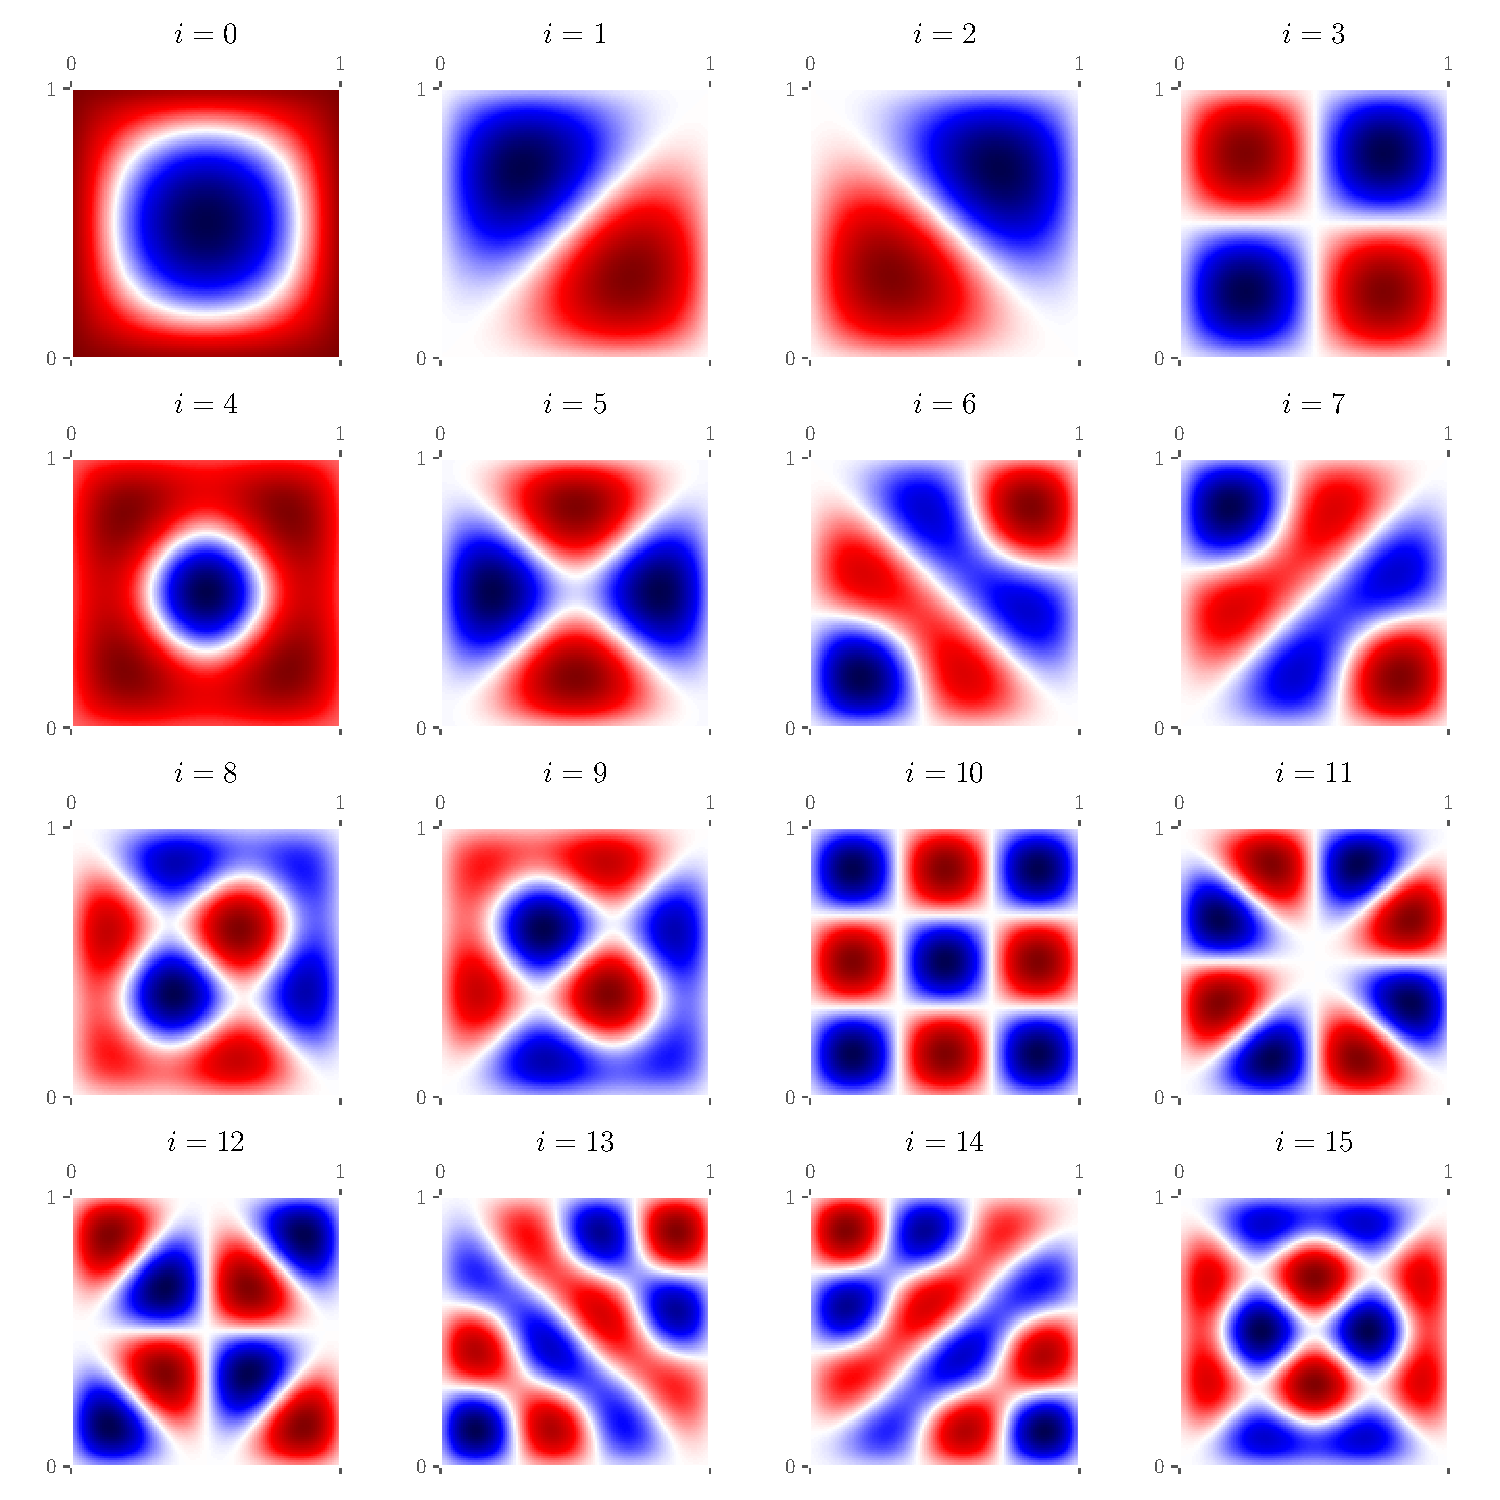
\includegraphics[width=0.7\textwidth]{1-0-nihajni_nacini_sparse.pdf}
\end{center}
Nadaljeval sem z implementacijo potenčne metode. Sprva mi je nekaj težav predstavljala normalizacija lastnih vektorjev, a mi je kasneje uspelo:

\begin{center}
    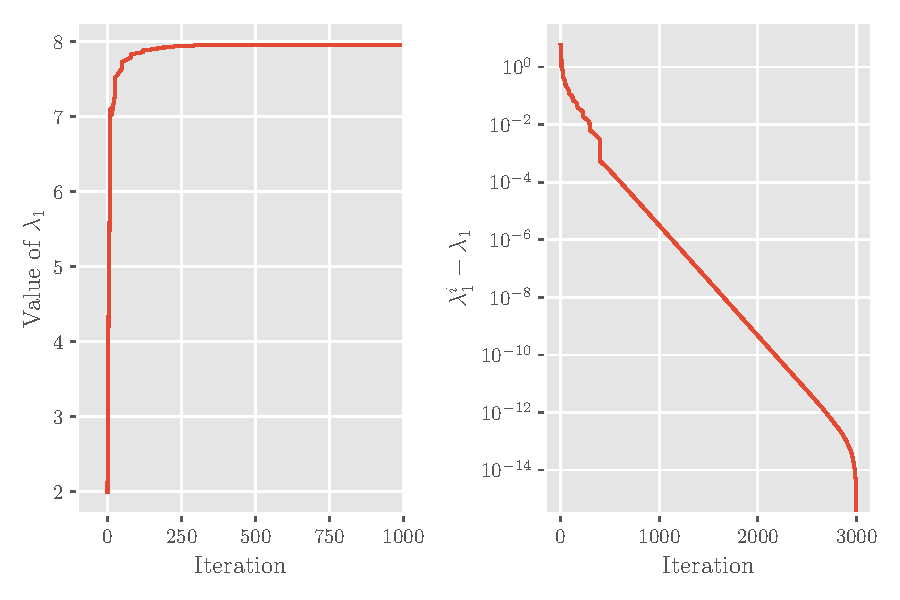
\includegraphics[width=0.8\textwidth]{1-0-powermethod.pdf}
\end{center}

Naslednji korak je nadgradnja metode za konvergenco k poljubni lastni vrednosti. Opazim, da zaradi iskanja inverza matrike $A - \sigma I$ potrebujem mnogo več časa za enako število iteracij. Optimizacija z knjižnjico \texttt{numba.jit} ni uspela.  Pri generaciji spodnje slike sem uporabil začetni približek $\lambda = 8$ in dosegel isto lastno vrednost kot prej. Poleg potrebe po invertiranju matrike vsako iteracijo algoritem dodatno podaljša tudi dejstvo, da je $\mathcal{O}$ metode po \cite{wiki} enak
\[\left| \frac{\sigma - \lambda_{\text{iskana}}}{\lambda_{\text{ naslednja najbližja}} - \lambda_{\text{iskana}}} \right|\]

\begin{center}
    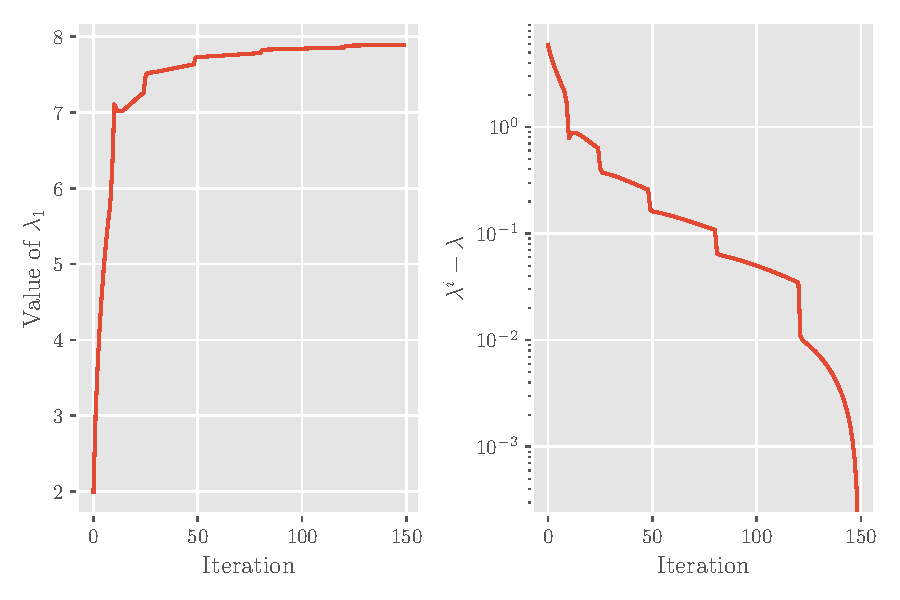
\includegraphics[width=0.8\textwidth]{1-0-inverse_powermethod.pdf}
\end{center}

Če inverzno potenčno metodo uporabim na razponu od 0 do maksimalne lastne vrednosti, dobim spodnjo sliko, ki nakazuje, da metoda ne deluje, kot bi si želeli.
\begin{center}
    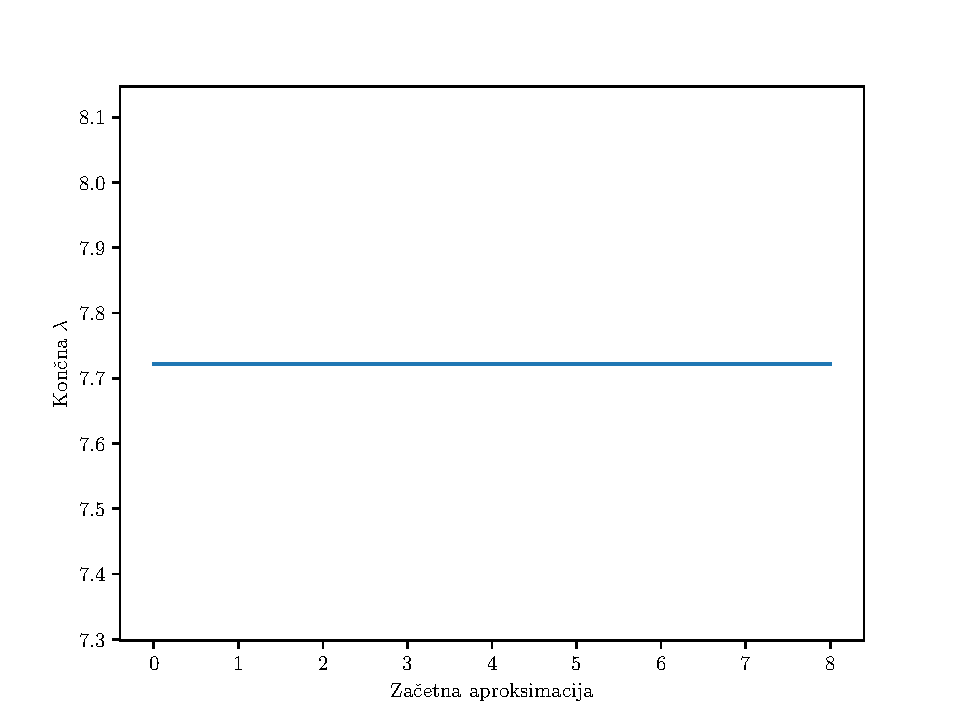
\includegraphics[width=0.7\textwidth]{1-0-inverse_powermethod_sweep.pdf}
\end{center}
V nadaljevanju sem zgeneriral zahtevano figuro:
\begin{center}
    
\includegraphics[width=0.5\textwidth]{1-figura.pdf}
\end{center}

Če dobljeno gostotno matriko $\rho(x,y)$ preoblikujemo v diagonalno matriko, jo lahko uporabimo v metodi \texttt{scipy.linalg.eigh} in izračunamo lastne vrednosti in lastne vektorje kot poprej:
\begin{center}
    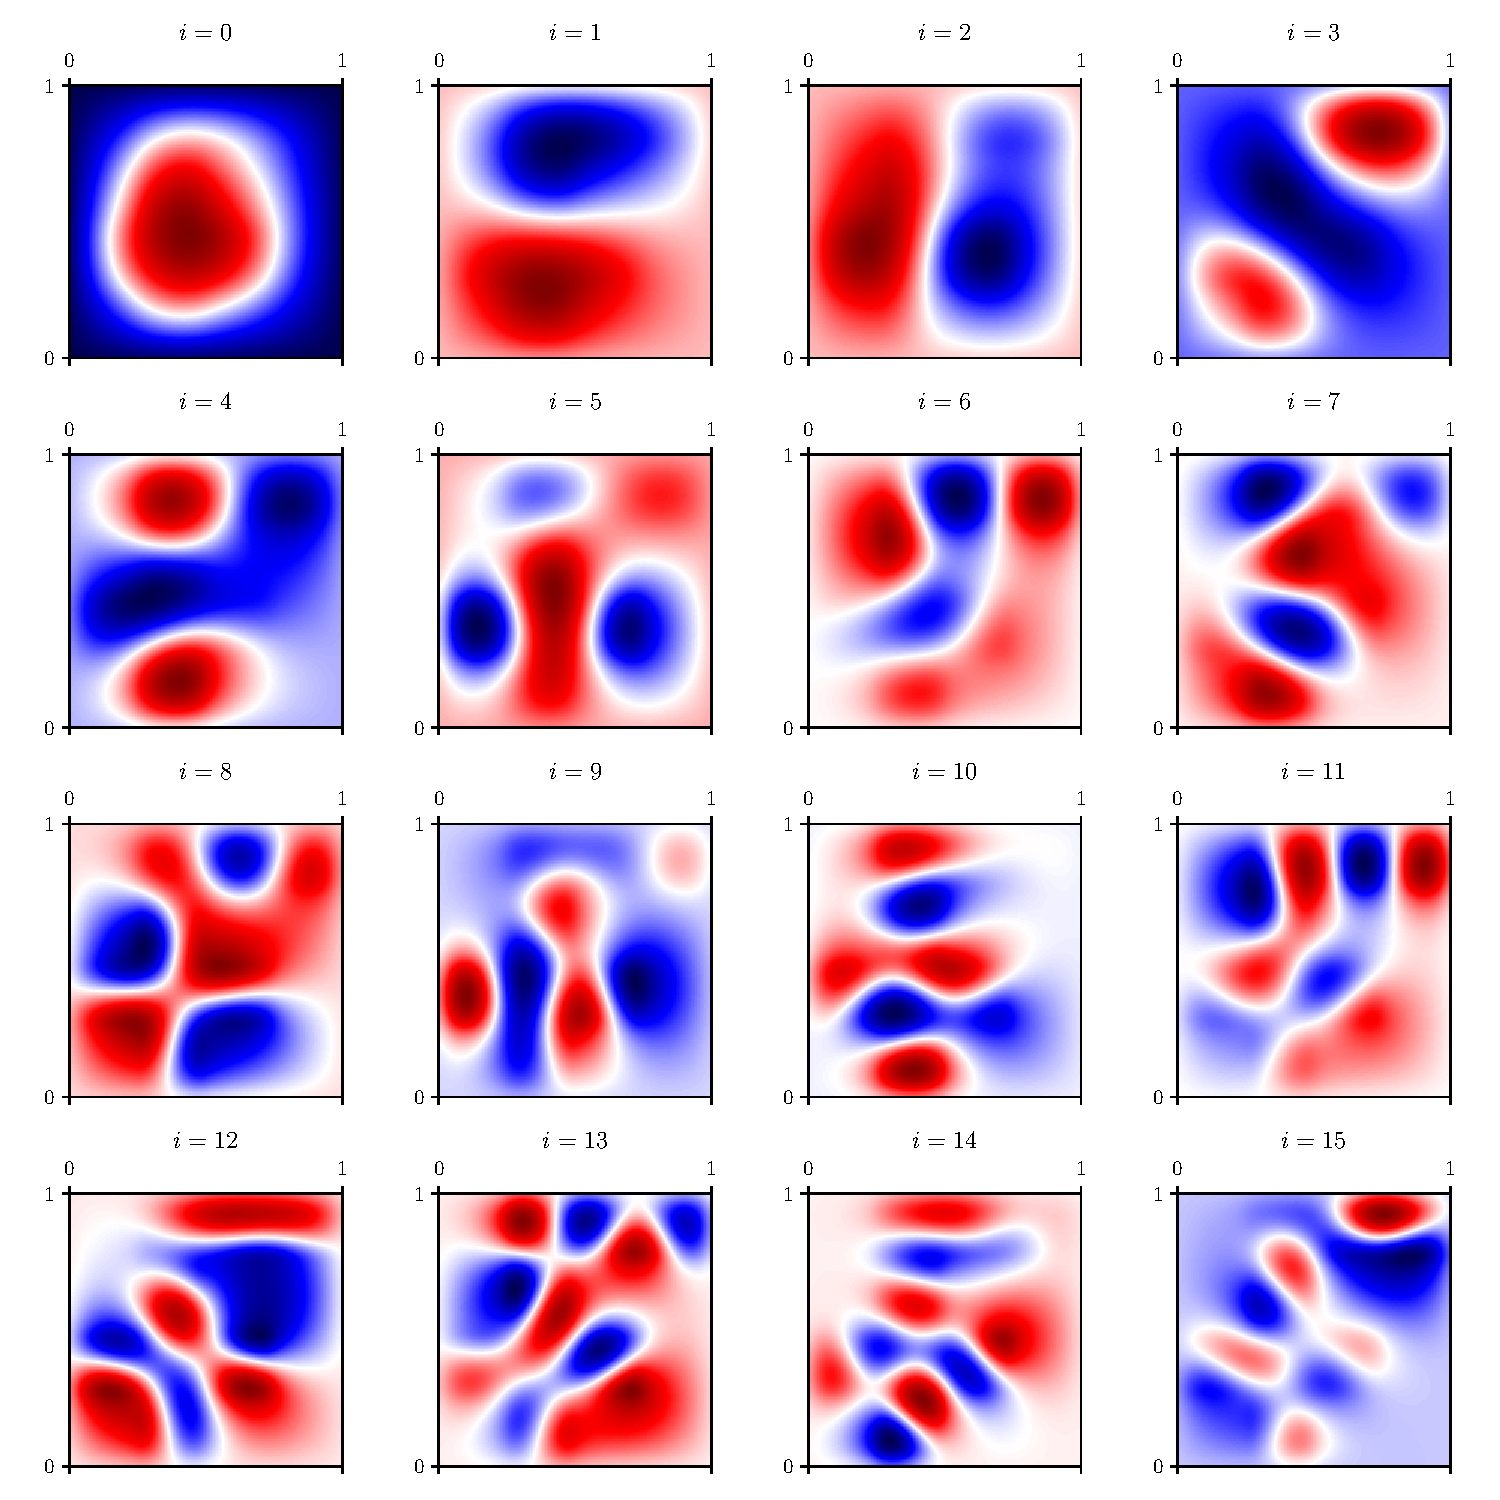
\includegraphics[width=\textwidth]{1-1-nihajni_nacini.pdf}
\end{center}
Prikazujem prvih 16 nihajnih načinov, uporabljeni gostoti sta 1 in 10, osenčena območja so tako manj gosta. Če gostoti zamenjam, dobim naslednjo sliko.
\begin{center}
    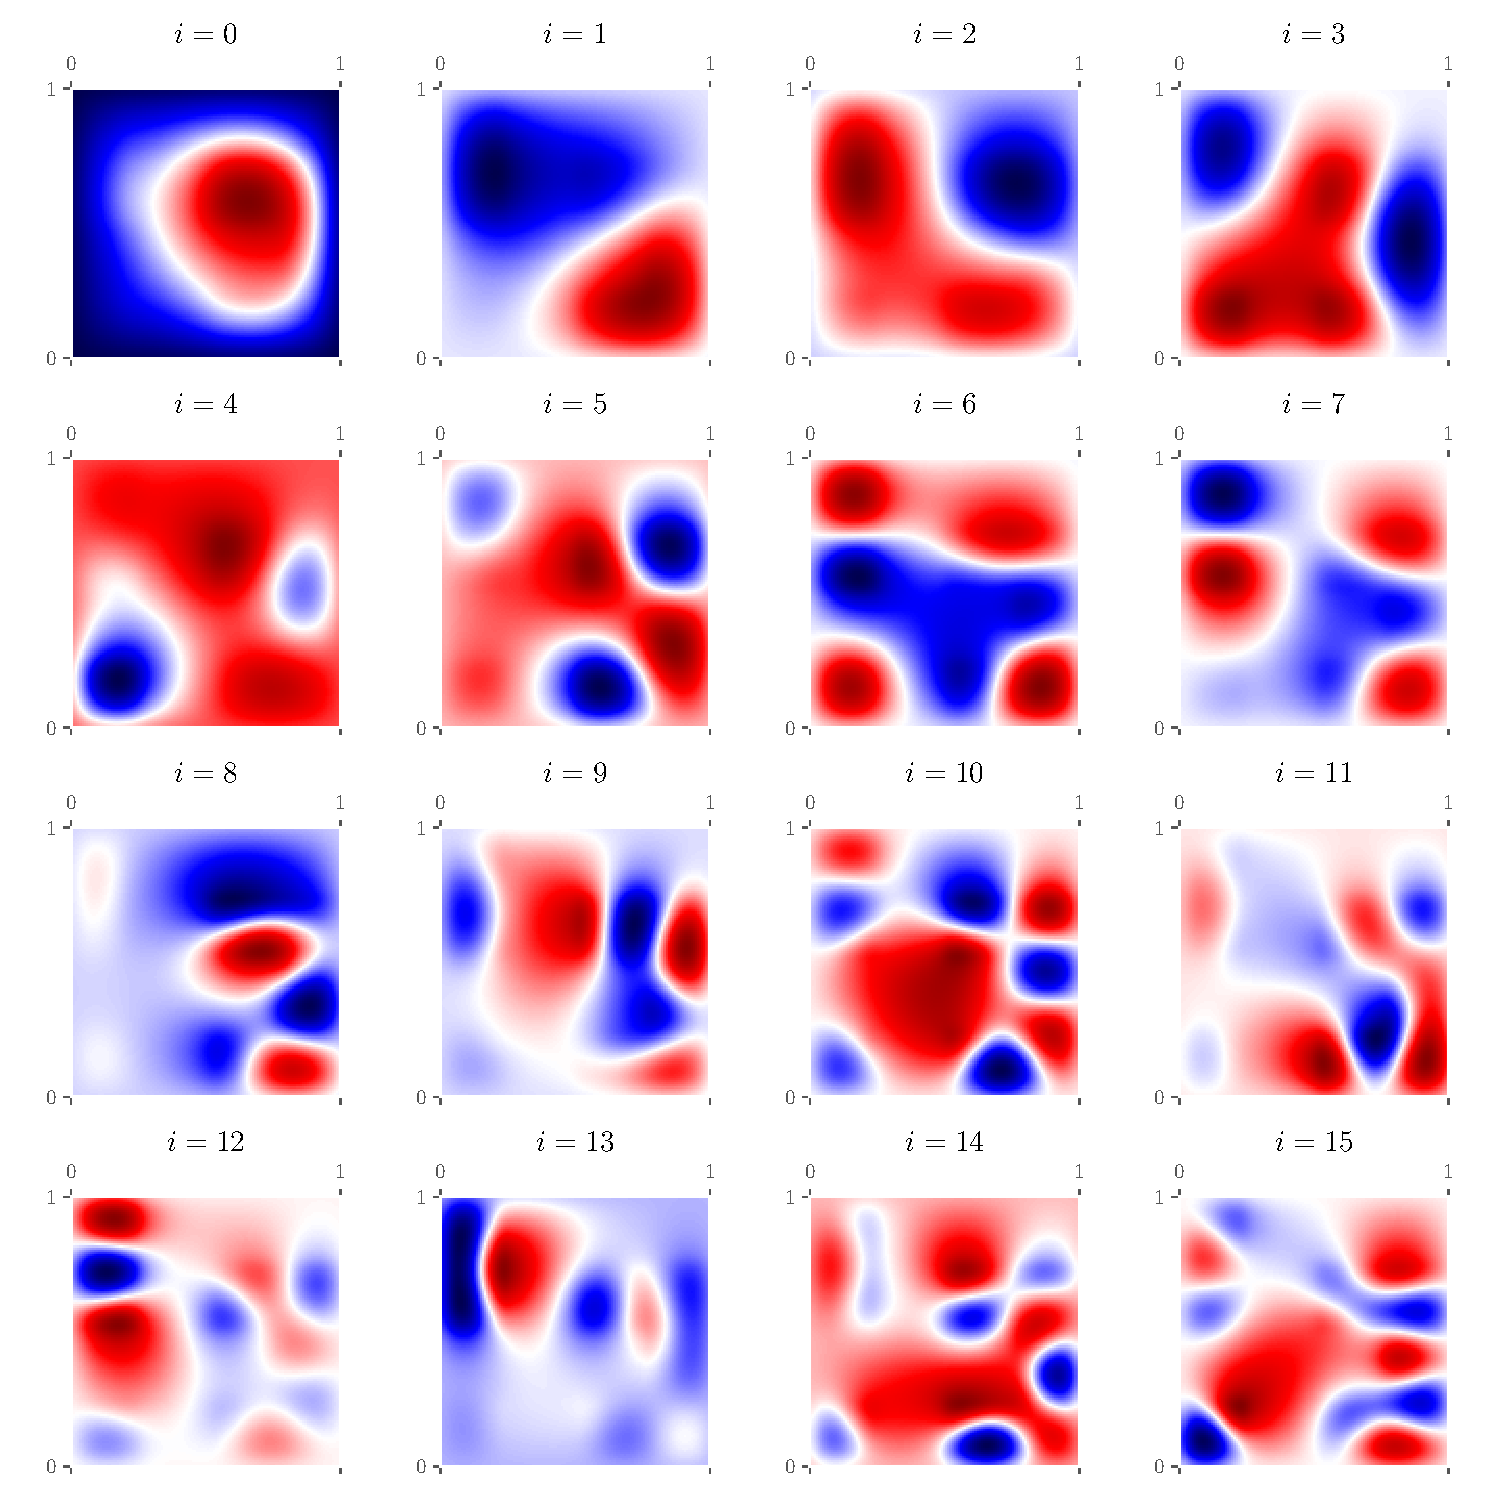
\includegraphics[width=\textwidth]{1-1-nihajni_nacini_inverted.pdf}
\end{center}
Poglejmo si še spekter obeh obtežitev, začenši z najnižjimi 16 lastnimi vrednostmi.
\begin{center}
    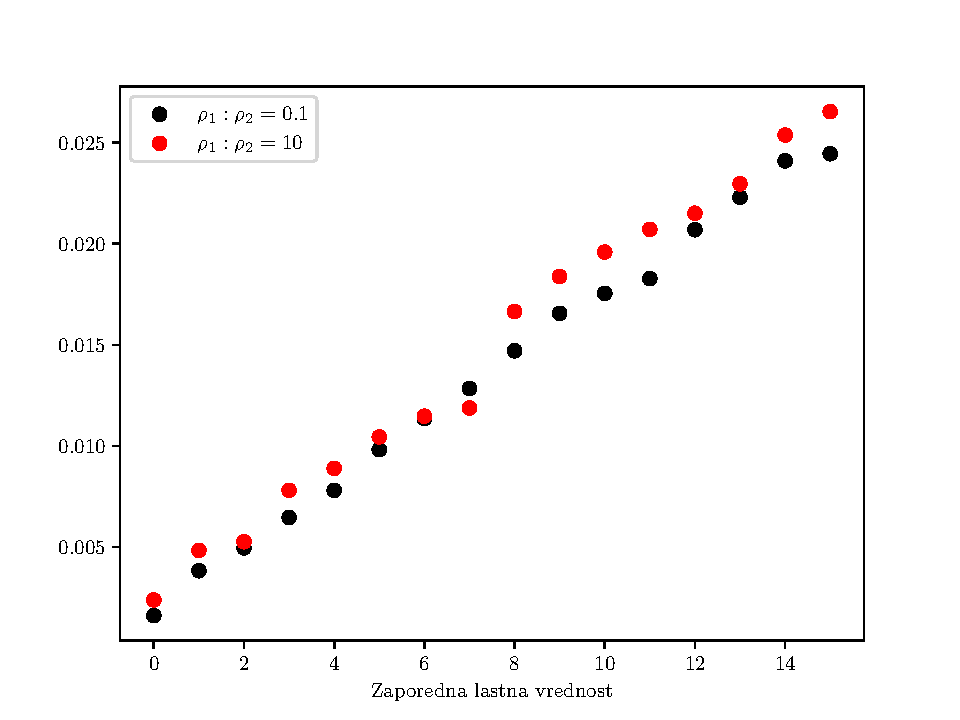
\includegraphics[width=\textwidth]{1-1-spekter-zoom_both.pdf}
\end{center}
Če pogledamo celoten spekter obeh obtežitev, dobimo spodnjo sliko.
\begin{center}
    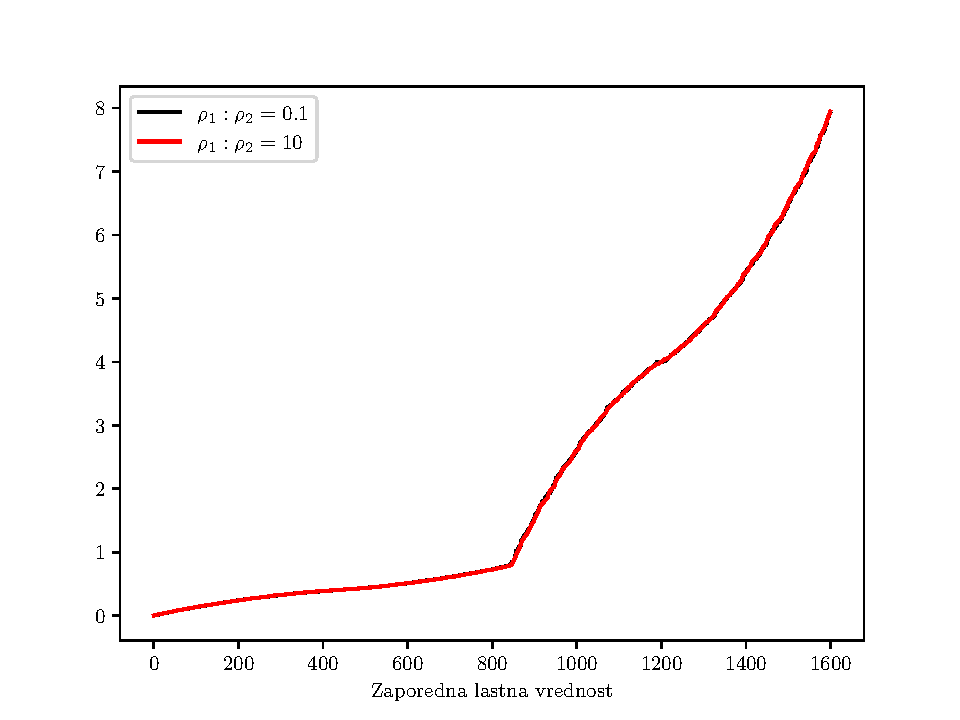
\includegraphics[width=\textwidth]{1-1-spekter_both.pdf}
\end{center}
Očitno je, da pride nekje na polovici do diskontinuitete, zato sem si ta prehod pogledal pobližje na še bolj ekstremnem razmerju gostot 1000:1. Najnižja lastna nihanja izgledajo presenetljivo podobna vsem ostalim:
\begin{center}
    \centering
        \begin{minipage}{0.45\textwidth}
        \centering
    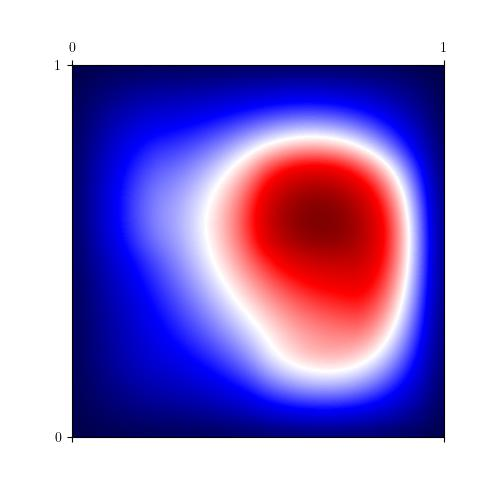
\includegraphics[width=\textwidth]{1-1-eigenmode-0.jpg}
    Prvi nihajni način za razmerje gostot 1000:1.
    \end{minipage}\hfill
    \begin{minipage}{0.45\textwidth}
        \centering
        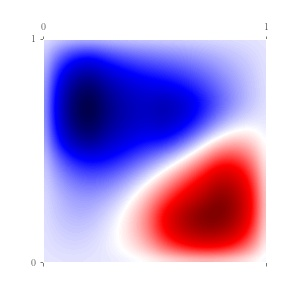
\includegraphics[width=1\textwidth]{1-1-eigenmode-1.jpg}
        Drugi nihajni način za isto opno.
    \end{minipage}
    \begin{minipage}{0.45\textwidth}
        \centering
    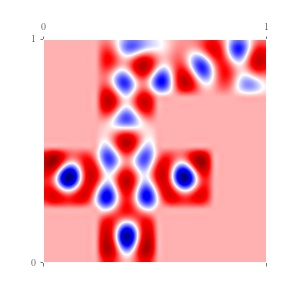
\includegraphics[width=\textwidth]{1-1-eigenmode-849.jpg}
    850. nihajni način za razmerje gostot 1000:1.
    \end{minipage}\hfill
    \begin{minipage}{0.45\textwidth}
        \centering
        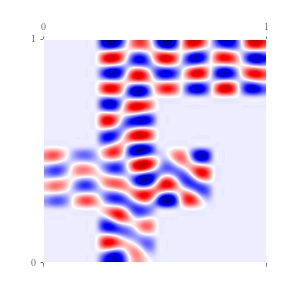
\includegraphics[width=1\textwidth]{1-1-eigenmode-900.jpg}
        901. nihajni način za isto opno.
    \end{minipage}
\end{center}
Postuliram, da zaradi diskontinuitete v spektru pride zaradi kvalitativno različnih nihanj; če prej celotna opna niha kot celota, po neki kritični lastni vrednosti težji deli opne obmirujejo, nihanje pa se z venomer večjimi valovnimi števili razvije v lažjem delu.


\section{}
Oceni lastne vrednosti operatorja $\nabla^{2}$ na problemu lastnih rešitev za polkrog z robnim pogojem
I. vrste.

\subsection{Reševanje}

Ponovno pripravim matriko, ki v diskretni obliki opisuje operator $\nabla^2$. Tokrat ni asimetrična, zato sem pri uporabi \texttt{scipy.sparse.linalg} našel kompleksne rešitve (sicer z imaginarno komponento, primerljivo z $\varepsilon_\text{machine}$). Z knjižnjico \texttt{scipy.linalg} teh problemov nisem imel, zato sem se posluževal slednje. Na podlagi rezultatov prve naloge pričakujem, da bi se metodi dobro ujemali in bo nadaljnje obnašanje rešitev podobno.

Ko sem lastne vektorje in vrednosti izračunal, sem si jih izrisal v polarni geometriji.

\begin{center}
    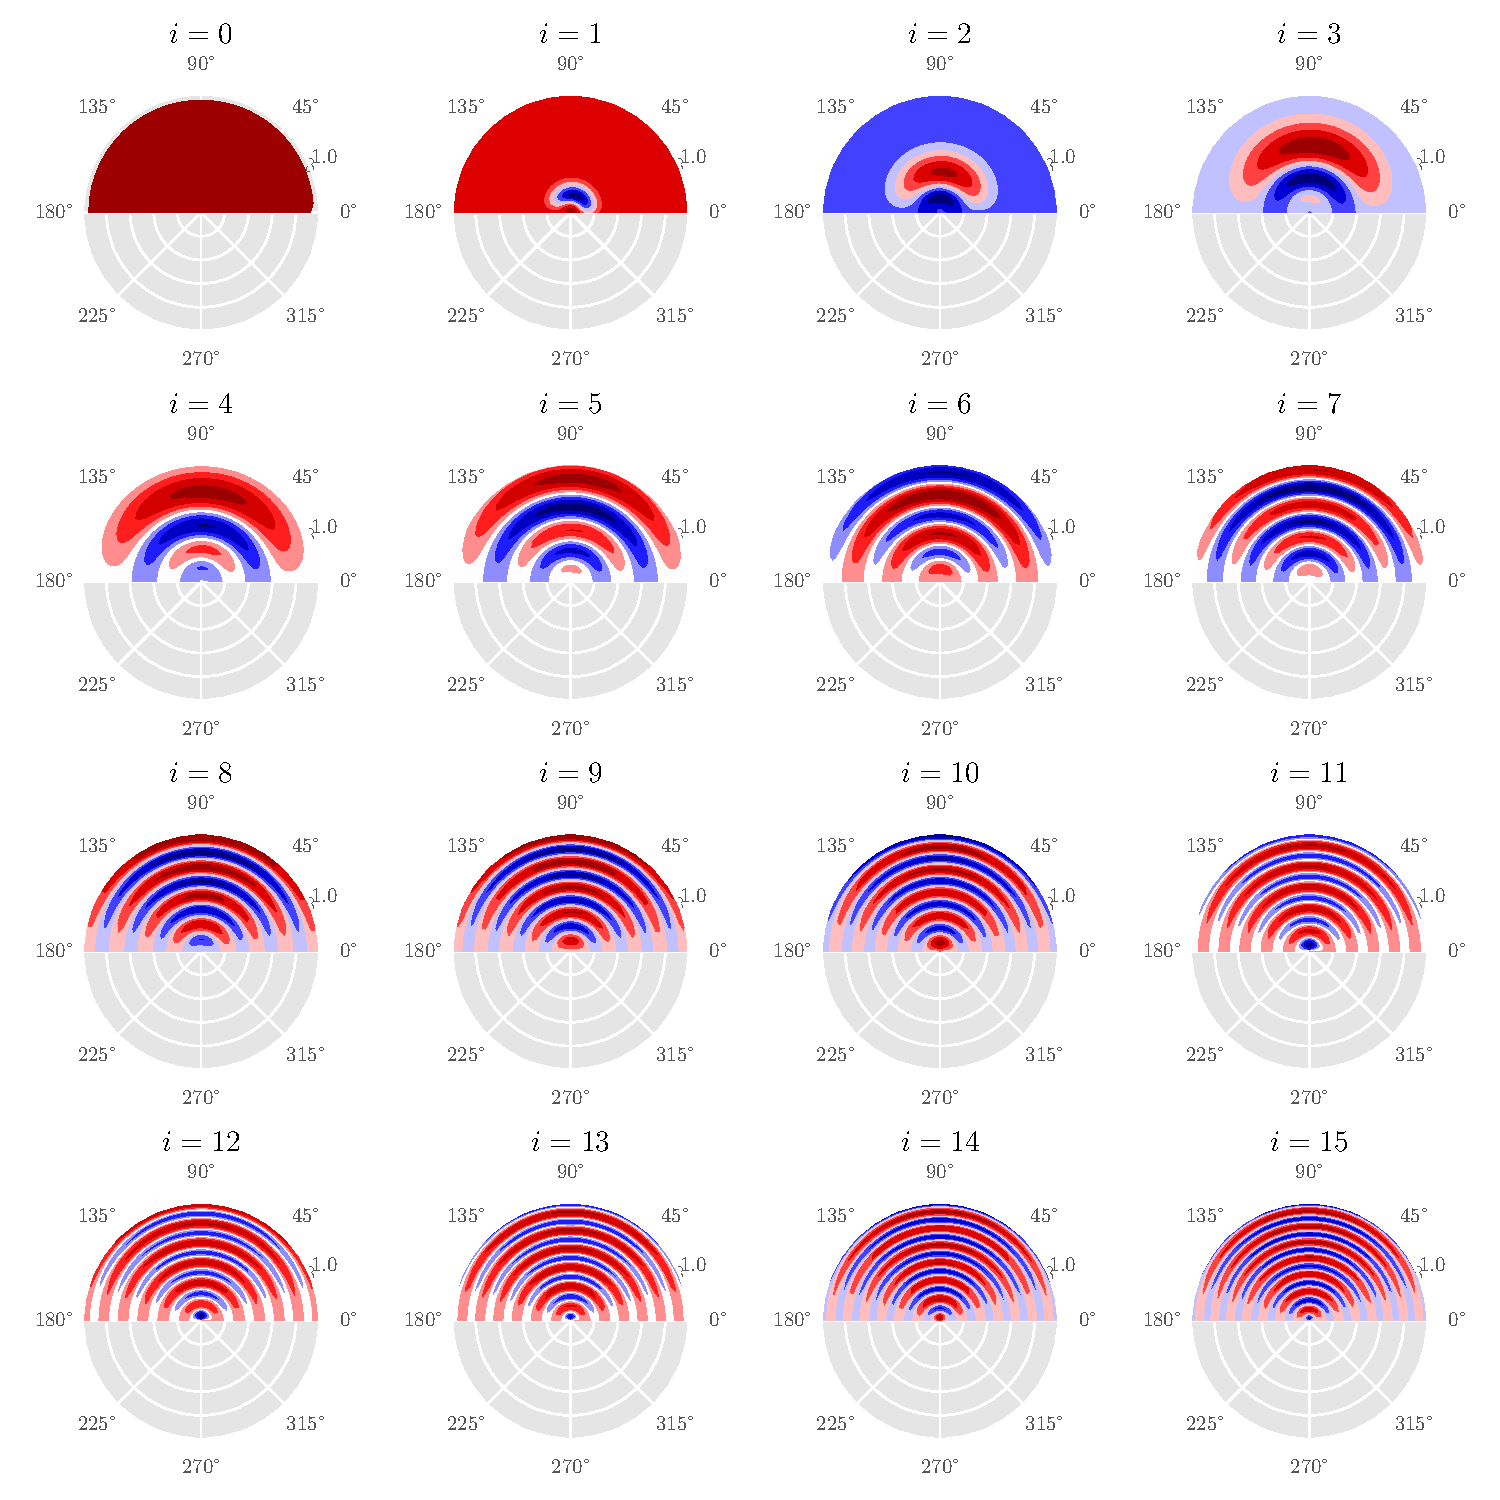
\includegraphics[width=0.9\textwidth]{2-nihajni_nacini.pdf}
\end{center}
Ker me je skrbelo, zakaj  ne vidim večje polarne odvisnosti, sem pogledal tudi višje lastne nihajne načine in se uveril, da dobim pričakovano obnašanje tudi po polarnem kotu.



\begin{center}
    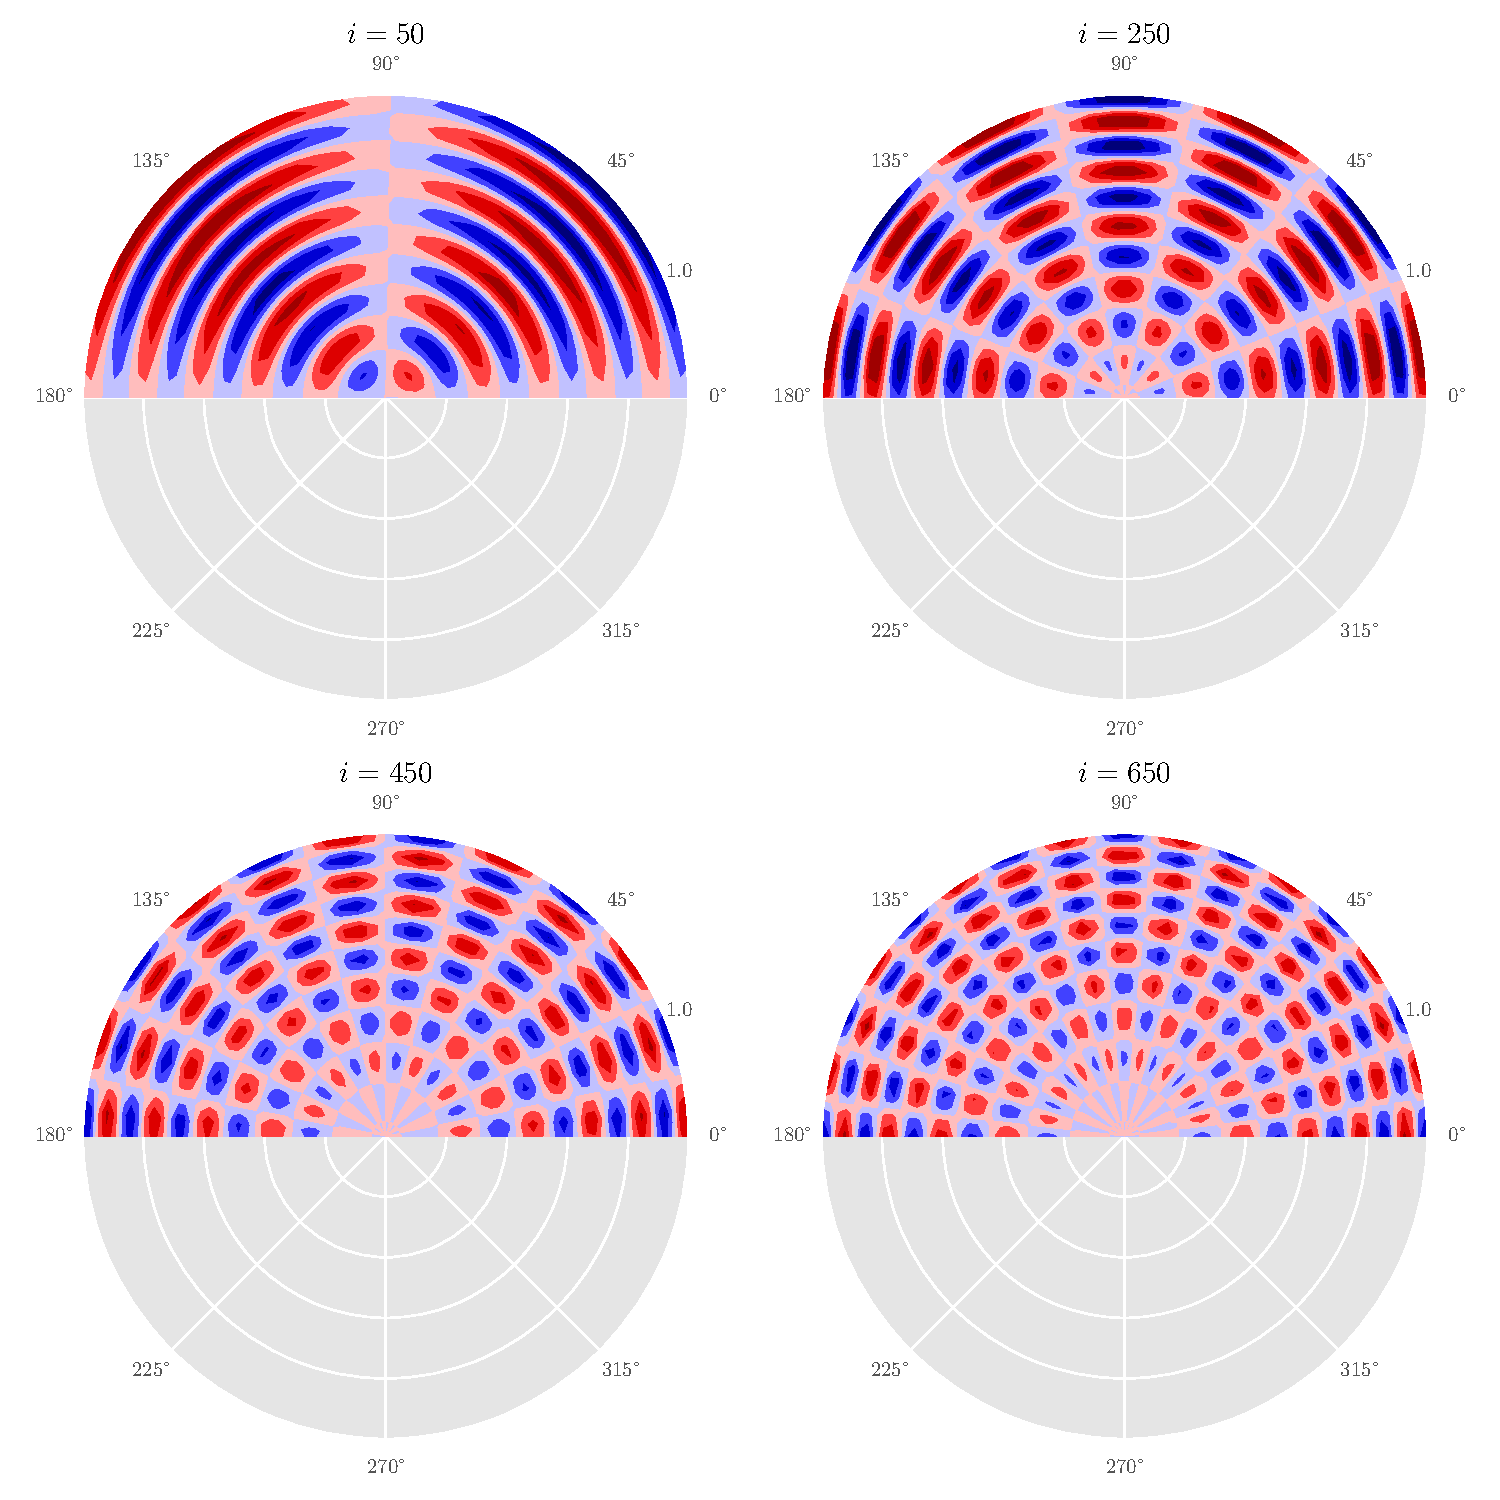
\includegraphics[width=0.8\textwidth]{2-nihajni_nacini_miks.pdf}
\end{center}
Spekter matrike, ki opisuje operator $\nabla^2$, prikazujem spodaj.
\begin{center}
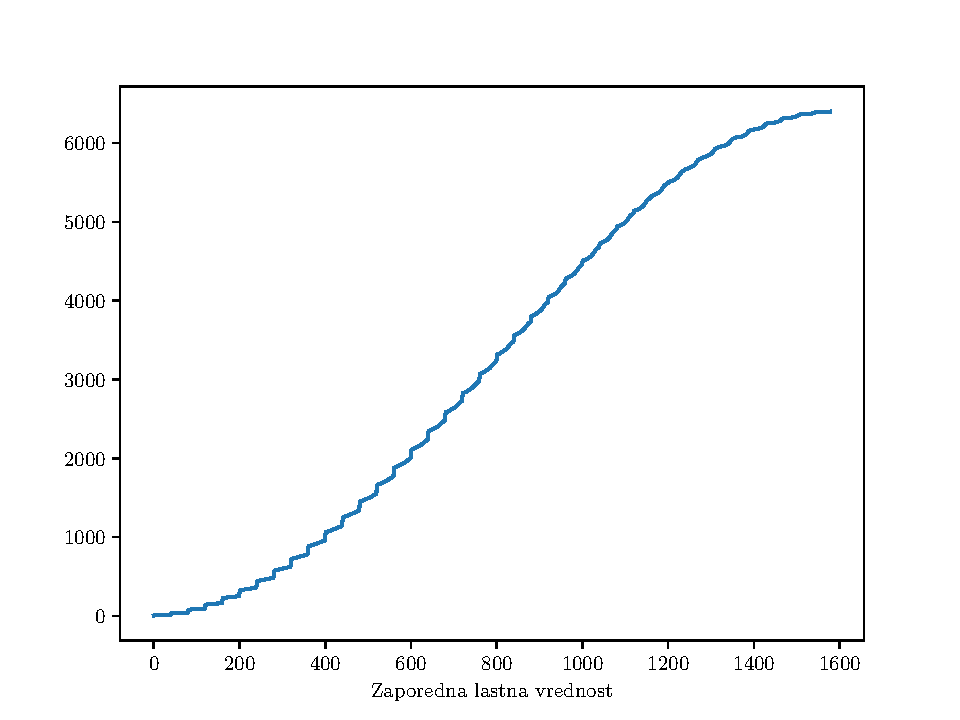
\includegraphics[width=0.7\textwidth]{2-spekter.pdf}
\end{center}


\begin{thebibliography}{9}
\bibitem{wiki} \url{https://en.wikipedia.org/wiki/Inverse_iteration}

\end{thebibliography}
\end{document}

\begin{figure}
    \centering
        \begin{minipage}{0.45\textwidth}
        \centering
    \includegraphics[width=\textwidth]{}
    \caption{}
        \label{fig:}
    \end{minipage}\hfill
    \begin{minipage}{0.45\textwidth}
        \centering
        \includegraphics[width=1\textwidth]{}
    \caption{}
    \label{fig:}
    \end{minipage}
\end{figure}
